\documentclass[12pt, titlepage]{article}

\usepackage{booktabs}
\usepackage{tabularx}
\usepackage[hidelinks]{hyperref}
\usepackage{amsfonts}
\usepackage{amssymb}
\usepackage{graphicx}
\usepackage{float}
\usepackage{colortbl}
\usepackage{xr}
\hypersetup{
    colorlinks,
    citecolor=black,
    filecolor=black,
    linkcolor=red,
    urlcolor=blue
}
\usepackage[round]{natbib}

%% Comments

\usepackage{color}

\newif\ifcomments\commentstrue %displays comments
%\newif\ifcomments\commentsfalse %so that comments do not display

\ifcomments
\newcommand{\authornote}[3]{\textcolor{#1}{[#3 ---#2]}}
\newcommand{\todo}[1]{\textcolor{red}{[TODO: #1]}}
\else
\newcommand{\authornote}[3]{}
\newcommand{\todo}[1]{}
\fi

\newcommand{\wss}[1]{\authornote{blue}{SS}{#1}} 
\newcommand{\plt}[1]{\authornote{magenta}{TPLT}{#1}} %For explanation of the template
\newcommand{\an}[1]{\authornote{cyan}{Author}{#1}}

%% Common Parts

\newcommand{\progname}{2D Localizer} % PUT YOUR PROGRAM NAME HERE
\newcommand{\authname}{Aliyah Jimoh} % AUTHOR NAMES                  

\usepackage{hyperref}
    \hypersetup{colorlinks=true, linkcolor=blue, citecolor=blue, filecolor=blue,
                urlcolor=blue, unicode=false}
    \urlstyle{same}
                                


\begin{document}

\title{Verification and Validation Report: \progname} 
\author{Aliyah Jimoh}
\date{\today}
	
\maketitle

\pagenumbering{roman}

\section{Revision History}

\begin{tabularx}{\textwidth}{p{3cm}p{2cm}X}
\toprule {\bf Date} & {\bf Version} & {\bf Notes}\\
\midrule
2024/04/18 & 1.0 & Initial Draft\\
% Date 2 & 1.1 & Notes\\
\bottomrule
\end{tabularx}

~\newpage

\section{Symbols, Abbreviations and Acronyms}

\renewcommand{\arraystretch}{1.2}
\begin{tabular}{l l} 
  \toprule		
  \textbf{symbol} & \textbf{description}\\
  \midrule 
  FM & Fiducial Marker\\
  T & Test\\
  SRS & Software Requirement Specification\\
  VnV & Verification and Validation\\
  \bottomrule
\end{tabular}\\

\newpage

\tableofcontents

\listoftables %if appropriate

\listoffigures %if appropriate

\newpage

\pagenumbering{arabic}

This document shows the results of the system and unit tests done on the \progname~software. More detailed information of the tests cases performed are documented in this system's \href{https://github.com/AliyahJimoh/2D-Localizer/blob/main/docs/VnVPlan/VnVPlan.pdf}{VnV Plan}.

\section{Functional Requirements Evaluation}

\subsection{Validate and Verify Inputs}
\begin{itemize}
  \item \textbf{Test Case(s): }\texttt{test\_map\_image}, \texttt{test\_coordinates}, \texttt{test\_range\_measurements}, \texttt{test\_invalid\_input}, \texttt{test\_nan\_beacon\_rejection}
  \item \textbf{Requirement(s) Met: }
  \begin{itemize}
    \item R1: Accept a map/image as an input
    \item R2: Accept sensor and fiducial marker (FM) coordinates as an input
    \item R3: Accept sensor measurements as an input
    \item R4: Verify that inputs provided are within their constraints
  \end{itemize}
  \item \textbf{Type: }Automatic
  \item \textbf{Testing Method: }\texttt{pytest}
  \item \textbf{Result Summary: }All 5 successfully passed
  \item \textbf{Result Location: }Unit tests from \texttt{test\_inputs\_results.txt} and \texttt{test\_input\_file\_results.txt} are located in the timestamp folder of \href{https://github.com/AliyahJimoh/2D-Localizer/tree/main/test/results/}{test/results}.
\end{itemize}


\subsection{Verify Localization}
\begin{itemize}
  \item \textbf{Test Case(s): }\texttt{test\_range\_only}, \texttt{test\_fiducials}, \texttt{test\_sensor\_fusion}
  \item \textbf{Requirement(s) Met: }
  \begin{itemize}
    \item R5: Compute estimated pose from provided inputs
  \end{itemize}
  \item \textbf{Type: }Automatic
  \item \textbf{Testing Method: }\texttt{pytest}
  \item \textbf{Result Summary: }All 3 successfully passed
  \item \textbf{Result Location: }Can all be found in \texttt{test\_pose\_estimation\_results.txt} located in the timestamp folder of \href{https://github.com/AliyahJimoh/2D-Localizer/tree/main/test/results/}{test/results}.
\end{itemize}

\subsection{Accuracy Evaluation}
\begin{itemize}
  \item \textbf{Test Case(s): }\texttt{test\_accuracy}
  \item \textbf{Requirement(s) Met: }
  \begin{itemize}
    \item R6: Evaluate the accuracy of the estimated pose with statistical models (found in \href{https://github.com/AliyahJimoh/2D-Localizer/blob/main/docs/SRS/SRS.pdf}{SRS})
  \end{itemize}
  \item \textbf{Type: }Automatic
  \item \textbf{Testing Method: }\texttt{pytest}
  \item \textbf{Result Summary: }Successfully passed
  \item \textbf{Result Location: }Can all be found in \texttt{test\_accuracy\_results.txt} located in the timestamp folder of the \href{https://github.com/AliyahJimoh/2D-Localizer/tree/main/test/results/}{results} folder.
\end{itemize}

\subsection{Validate Visualization}
\begin{itemize}
  \item \textbf{Test Case(s): }\texttt{test\_visualization}
  \item \textbf{Requirement(s) Met: }
  \begin{itemize}
    \item R7: Display visual representation (plot) of pose estimate
    \item R8: Display reat-time coordinate updates of the robot
    \item R9: Display the robot's trajectory path
  \end{itemize}
  \item \textbf{Type: }Automatic
  \item \textbf{Testing Method: }\texttt{pytest}
  \item \textbf{Result Summary: }Successfully passed. There are warnings that come up since the plot is being tested that it can display rather than actually displaying it.
  \item \textbf{Result Location: }Can all be found in \texttt{test\_visuals\_results.txt} located in the timestamp folder of \href{https://github.com/AliyahJimoh/2D-Localizer/tree/main/test/results/}{test/results}.
\end{itemize}

\section{Nonfunctional Requirements Evaluation}

\subsection{Accuracy}
\begin{itemize}
  \item \textbf{Test Case(s): }\texttt{test\_accuracy}
  \item \textbf{Requirement(s) Met: }
  \begin{itemize}
    \item NFR1: Ensure that the accuracy metric output by the system is numerically sound.
  \end{itemize}
  \item \textbf{Type: }Automatic
  \item \textbf{Testing Method: }\texttt{pytest}
  \item \textbf{Result Summary: }Successfully passed
  \item \textbf{Result Location: }Can all be found in \texttt{test\_accuracy\_results.txt} located in the timestamp folder of the \href{https://github.com/AliyahJimoh/2D-Localizer/tree/main/test/results/}{results} folder.
\end{itemize}
		
\subsection{Maintainability}
\begin{itemize}
  \item \textbf{Requirement(s) Met: }
  \begin{itemize}
    \item NRF2: Software should be simple to modify some components when
    needed.
  \end{itemize}
  \item \textbf{Type: }Manual
  \item \textbf{Testing Method: }Modifying components in modules and rerunning the unit tests in pytest to see if \progname~still works.
  \item \textbf{Result Summary: }Software still operational.
\end{itemize}

\subsection{Usability}
\begin{itemize}
  \item \textbf{Requirement(s) Met: }
  \begin{itemize}
    \item NFR3: Software should be able to run on Linux operating systems and macOS.
  \end{itemize}
  \item \textbf{Type: }Manual
  \item \textbf{Testing Method: }Running the \texttt{make install} command from the Makefile found in the src folder using two laptops (one with Linux and the other with macOS)
  \item \textbf{Result Summary: }Both laptops were successfully able to install the virtual environment and run the software.
\end{itemize}
	
\section{Comparison to Existing Implementation}	

This section is not applicable.

\section{Unit Testing}

The unit tests for \progname~are run using the command \texttt{make\ test} which executes the program \texttt{unit\_tests.py} located in the test folder. The script looks through all the programs that start with `test\_' and end with `.py' as that is the naming convention that was chosen for all test cases. 

After all the tests finish running, the program generates a .txt summary file each module tested. This file records whether the test passed or failed and indicates the location where the result is stored. A combined terminal output also provides a quick summary of the results.

\begin{figure}[H]
  \centering
  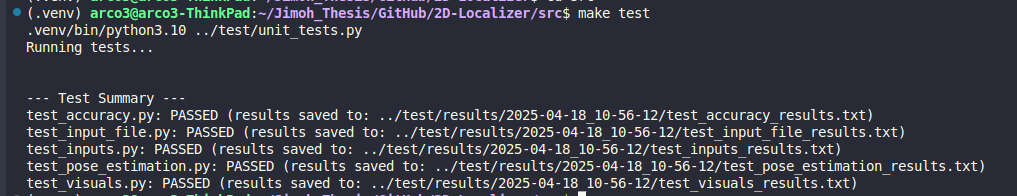
\includegraphics[width=1\textwidth]{make_test.png}
  \caption{Output of the make test command}
\end{figure}

\begin{figure}[H]
  \centering
  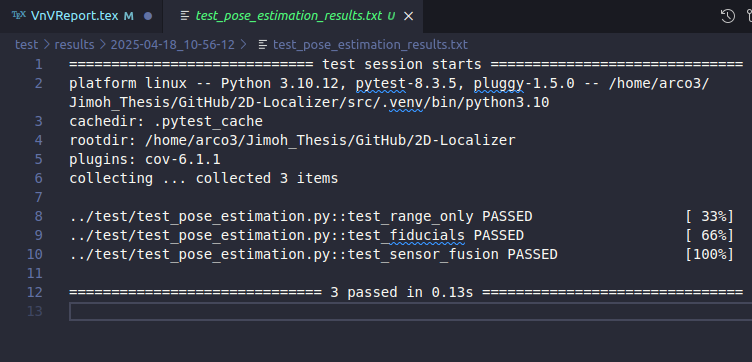
\includegraphics[width=1\textwidth]{test_summary.png}
  \caption{Test Summary for test\_pose\_estimation.py}
\end{figure}

\section{Changes Due to Testing}

% \wss{This section should highlight how feedback from the users and from 
% the supervisor (when one exists) shaped the final product.  In particular 
% the feedback from the Rev 0 demo to the supervisor (or to potential users) 
% should be highlighted.}

\begin{itemize}
  \item \textbf{Improved Accuracy Validation:} The approach for evaluating pose accuracy was expanded. The final version includes explicit tests for Fisher Information Matrix (FIM) and Cramér-Rao Lower Bound (CRLB), validated in \texttt{test\_accuracy.py}.

  \item \textbf{Expanded Unit Testing and Coverage:} Initial versions of the VnV Plan lacked specific testing for key modules such as plotting and input validation. These were added in \texttt{test\_visuals.py} and \texttt{test\_inputs.py}, respectively.

  \item \textbf{Integration with Automation Tools:} To support repeatable testing, automated testing was introduced through an extra command in the Makefile to output summaries. This ensures that changes to the codebase can be quickly validated after updates.
\end{itemize}

\section{Automated Testing}

All unit and system tests were written using the \texttt{pytest} framework. Test scripts followed a consistent \texttt{test\_*.py} naming convention and were validated using both standalone runs and automated workflows. This custom Python script, \texttt{unit\_tests.py}, automatically discovers all test files and records their output in corresponding \texttt{.txt} summary files the \href{https://github.com/AliyahJimoh/2D-Localizer/tree/main/test/results}{test/results} folder in the GitHub Repository.

		
\section{Trace to Requirements}
\begin{table}[H]
  \begin{center}
    \resizebox{1.1\textwidth}{!}{ 

    \begin{tabular}{|l|c|c|c|c|c|c|c|c|c|c|}
    \hline
    \multicolumn{1}{|c|}{\textbf{Test Case}} &
      \textbf{R1} &
      \textbf{R2} &
      \textbf{R3} &
      \textbf{R4} &
      \textbf{R5} &
      \textbf{R6} &
      \textbf{R7} &
      \textbf{R8} &
      \textbf{R9} &
      \textbf{NFR1} \\ \hline
    test\_invalid\_yaml       &   &   &   & X &   &   &   &   &   &   \\
    test\_map\_image          & X &   &   &   &   &   &   &   &   &   \\
    test\_coordinates         &   & X &   &   &   &   &   &   &   &   \\
    test\_range\_measurements &   &   & X &   &   &   &   &   &   &   \\ \hline
    test\_range\_only         &   &   & X &   &   &   &   &   &   &   \\
    test\_fiducials           &   & X &   &   &   &   &   &   &   &   \\
    test\_sensor\_fusion      &   & X & X &   & X &   &   &   &   &   \\ \hline
    test\_visualization       &   &   &   &   &   &   & X & X & X &   \\ \hline
    test\_accuracy            &   &   &   &   &   & X &   &   &   & X \\ \hline
    \end{tabular}
  }
  \caption{Tracibility Matrix Between the Test Cases \& Requirements}
  \end{center}
  \end{table}
		
\section{Trace to Modules}	
\begin{table}[H]
  \centering
  \resizebox{1.1\textwidth}{!}{
    \begin{tabular}{|l|c|c|c|c|}
      \hline
      \multicolumn{1}{|c|}{\textbf{Test Case}} & \textbf{localization.py} & \textbf{input\_format.py} & \textbf{accuraccy.py} & \textbf{plot.py} \\ \hline
      test\_invalid\_yaml       &   & X &   &   \\ \hline
      test\_map\_image          &   & X &   &   \\ \hline
      test\_coordinates         &   & X &   &   \\ \hline
      test\_range\_measurements &   & X &   &   \\ \hline
      test\_range\_only         & X &   &   &   \\ \hline
      test\_fiducials           & X &   &   &   \\ \hline
      test\_sensor\_fusion      & X &   &   &   \\ \hline
      test\_visualization       &   &   &   & X \\ \hline
      test\_accuracy            &   &   & X &   \\ \hline
    \end{tabular}
  }
  \caption{Tracibility Matrix Between the Test Cases \& Modules}
  \end{table}	

\section{Code Coverage Metrics}

As mentioned in the \href{https://github.com/AliyahJimoh/2D-Localizer/blob/main/docs/VnVPlan/VnVPlan.pdf}{VnV Plan}, there were some modules that were justified for not having any unit tests resulting in their coverage being 0\%. Due to this, the main focus will be the coverage:
\begin{itemize}
  \item Input Format Module (M3)
  \item Localization Module (M6)
  \item Plotting Module (M8)
  \item Accuracy Evaluation Module (M9)
\end{itemize}

\begin{table}[H]
  \begin{center}
  \begin{tabular}{ |c|c|c|c| }
  \hline
   \textbf{Name} &  \textbf{Stmts} &  \textbf{Miss} &  \textbf{Coverage}\\ 
  \hline
  
      accuracy.py & 15 & 0 & 100\% \\ 
      \hline
      input\_format.py & 52 & 2 & 92\% \\
      \hline
      localization.py & 38 & 0 & 100\% \\ 
      \hline
      plot.py & 62 & 20 & 68\% \\
  \hline
  \end{tabular}
  \caption{Code Coverage Metric for the Unit Tested Modules}
\label{tab:code-coverage-metrics}
\end{center}
\end{table}

From what is being prioritized, all modules have a with over 60\%. The rationale for the Plotting Module being relatively low is due to the unit test not showing the plot but rather confirming that it can display and update itself.


\newpage
\bibliographystyle{plainnat}
\bibliography{../../refs/References}

\newpage{}

The information in this section will be used to evaluate the team members on the
graduate attribute of Reflection.

\begin{enumerate}
  \item What went well while writing this deliverable? 
  \item What pain points did you experience during this deliverable, and how
    did you resolve them?
  \item Which parts of this document stemmed from speaking to your client(s) or
  a proxy (e.g. your peers)? Which ones were not, and why?
  \item In what ways was the Verification and Validation (VnV) Plan different
  from the activities that were actually conducted for VnV?  If there were
  differences, what changes required the modification in the plan?  Why did
  these changes occur?  Would you be able to anticipate these changes in future
  projects?  If there weren't any differences, how was your team able to clearly
  predict a feasible amount of effort and the right tasks needed to build the
  evidence that demonstrates the required quality?  (It is expected that most
  teams will have had to deviate from their original VnV Plan.) \cite{Barfoot2017}
\end{enumerate}

\end{document}